%!TEX TS-program = xelatex
\documentclass[twoside]{article}

\usepackage{listings}
\usepackage{amsmath}
\usepackage{amsfonts}
\usepackage{graphicx}
\usepackage{multirow}
\usepackage{fontspec}
\usepackage{hyperref}
\usepackage{xepersian}

% Graphic Settings ===================
% Font Settings ======================
\setlatintextfont{LinLibertine}[Path = fonts/latin/]
\settextfont{HMXKayhan}[
Path = fonts/fa/ ,
BoldFont = HMXKayhanBd]
\graphicspath{{images/}}
\DeclareGraphicsExtensions{.jpeg,.png,.jpg}

\title{\Huge گزارش آزمایش 3 آز معماری کامپیوتر }
\author{\Large گروه 2}
\date{\Large امیرحسین علمدار - محمدپیام تائبی - ماهان بیهقی}

\begin{document}
	\maketitle
	\newpage
	\section*{نام آزمایش}
	جمع کننده/تفریق کننده ممیز شناور
	\section*{اهداف آزمایش}
	طراحی مدار جمع کننده و تفریق کننده برای اعداد ممیز شناور 12 بیتی
	
	\section*{شرح آزمایش}
	مدار جمع کننده طراحی شده ورودی های ممیز شناور A و B و سیگنال های کنترلی ADD/SUB و START دارد. با فعال شدن سیگنال START محاسبه آغاز میشود و پس از محاسبه حاصل جمع یا تفریق دو عدد A و B بسته به سیگنال کنترلی عملیات، حاصل عملیات را روی خروجی قرار داده و سیگنال کنترلی END هم یک میشود. در صورت وقوع اورفلو در فرایند جمع نیز سیگنال خروجی OVERFLOW یک میشود. مجدد با غیرفعال شدن سیگنال START مدار آماده دریافت مقادیر جدید میشود. همچنین ورودی ADD برای تعیین نوع عملیات مورد استفاده قرار میگیرد. در صورت 1 بودن این سیگنال حاصل A+B محاسبه میشود و در غیر این صورت مقدار A-B محاسبه میشود.
	در این آزمایش از اعداد 12 بیتی ممیز شناور که به فرمت زیر میباشند استفاده خواهیم کرد:
	\begin{figure}[h!]
		\begin{center}
			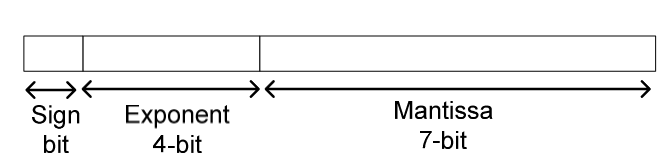
\includegraphics[scale=0.4]{format}‎
			\caption{فرمت 12 بیتی ورودی های و خروجی ها}
		\end{center}
	\end{figure} 
	
	\begin{figure}[h!]
		\begin{center}
			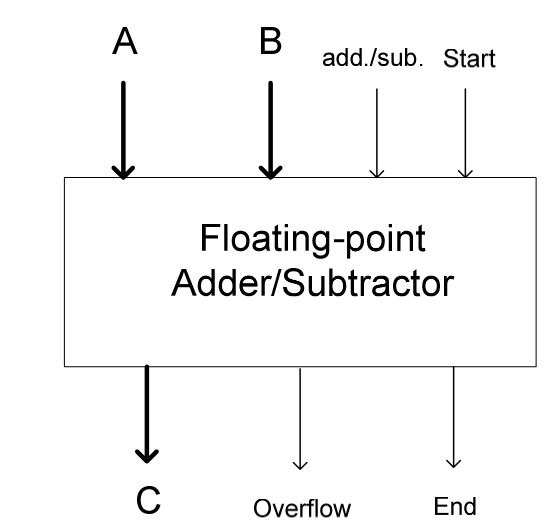
\includegraphics[scale=0.4]{blackbox}‎
			\caption{طرح بلک باکس مدار}
		\end{center}
	\end{figure} 

	\newpage
	\subsection*{مراحل آزمایش و مدارات}
	\subsection*{الگوریتم جمع و تفریق}	
	برای جمع و تفریق دو عدد ممیز شناور الگوریتم زیر را پیاده سازی میکنیم:
	\begin{itemize}
		\item 
		ورودی که نمای کوچکتری دارد را انقدر به راست شیفت میدهیم تا نمای هر دو عدد برابر شود.
		\item
		مقادیر عددی ورودی ها را با هم جمع میکنیم. در صورتی که هرکدام از اعدا منفی باشند، از مکمل دوی آن ها استفاده میکنیم. همچنین اگر عمیلات خواسته شده تفریق باشد، ورودی دوم را مکمل 2 میکنیم.
		\item
		وقوع اورفلو در جمع را بررسی میکنیم و نما را در صورت نیاز یک واحد افزایش میدهیم.
		\item
		 مقدار حاصل از جمع را نرمالایز میکنیم به گونه ای که در صورت امکان، بیت پرارزش خروجی 1 باشد. در این صورت مقدار نما را به اندازه ای کاهش میدهیم که تغییری در مقدار نهایی ایجاد نشود. اگر عدد دینرمالایز یا 0 باشد، نمای خروجی 0 خواهد بود.
	\end{itemize}
	\subsection*{طراحی شماتیک مدار}
	\begin{itemize}
		\item
		ورودی های مدار در هنگام محاسبه نباید تاثیری در محاسبه داشته باشند. برای پیاده سازی این ویژگی از قرار دادن لچ-D بر سر راه ورودی ها استفاده کرده ایم. با 1 شدن سیگنال START ورودی ها وارد مدار میشوند و محاسبه آغاز میشود.
			\begin{figure}[h!]
			\begin{center}
				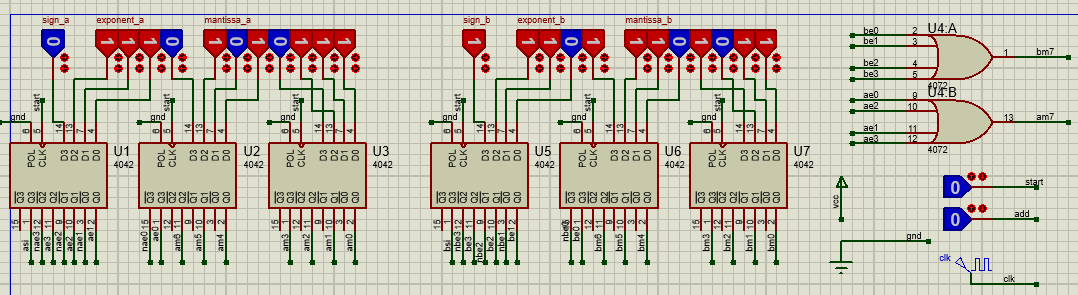
\includegraphics[scale=0.5]{inputs}‎
				\caption{ورودی های مدار}
			\end{center}
		\end{figure} 
		\item
		طبق الگوریتمی که در بالا معرفی شد به شیفترهای 8 بیتی با چهار ورودی SHAMT نیاز خواهیم داشت که مقدار شیفت را مشخص کند. برای طراحی این شیفترها از ساختار مدار ترکیبی شیفت دهنده بشکه ای استفاده میکنیم. البته شیفتر مورد نیاز در این سوال چهار ورودی کنترل کننده مقدار شیفت خواهد داشت تا جمع اعداد نرمالایز و دینرمالایز را هم پیاده سازی کند.	مدار طراحی شده برای این شیفتر به صورت زیر است :
		\begin{figure}[h!]
			\begin{center}
				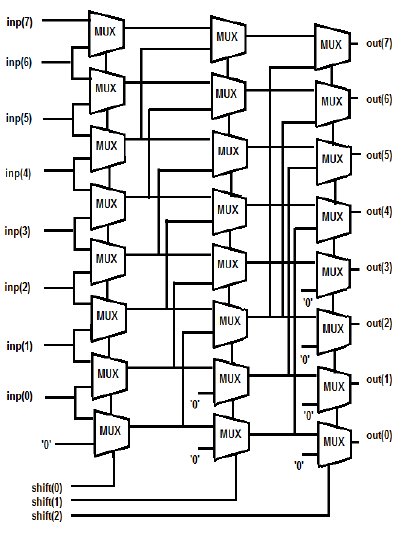
\includegraphics[scale=0.2]{barrel_shifter}‎
				\caption{شیفتر بشکه ای}
			\end{center}
		\end{figure} 
		\begin{figure}[h!]
			\begin{center}
				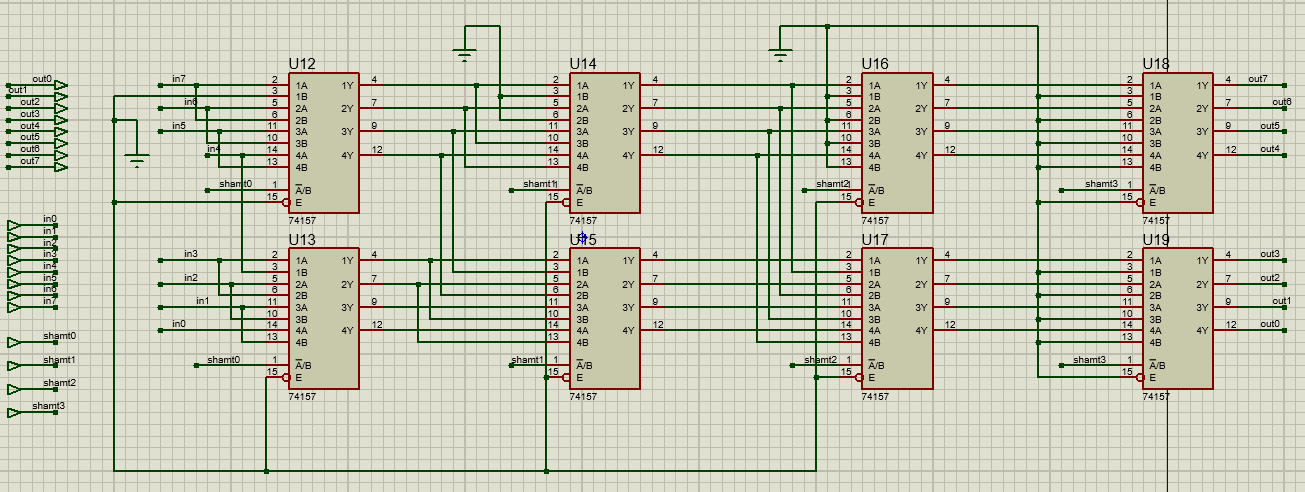
\includegraphics[scale=0.4]{barrel_shifter_circuit}‎
				\caption{شیفتر بشکه ای طراحی شده}
			\end{center}
		\end{figure} 
		\item
		حال که شیفتر را طراحی کرده ایم با مقایسه نماهای دو عدد، عدد کوچکتر را به اندازه اختلاف نماها به سمت راست شیفت میدهیم. مدار زیر این عملیات را نشان میدهد :
		\begin{figure}[h!]
			\begin{center}
				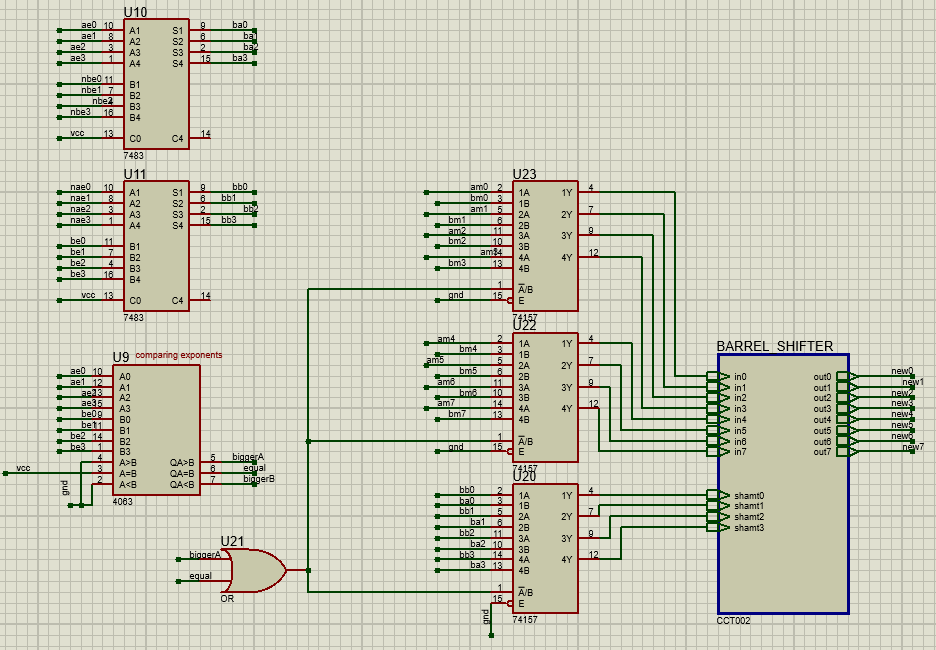
\includegraphics[scale=0.4]{shifting_lesser_number_circuit}‎
				\caption{ابتدا با یک مقایسه کننده دو نما مقایسه میشوند.سپس اختلاف نما ها محاسبه میشود و عدد کوچکتر به اندازه اختلاف نما شیفت داده میشود.}
			\end{center}
		\end{figure} 
		\newpage
		\item
		مدار جابه جا کننده زیر ورودی کوچک تر که شیفت داده شده است را در گاه صحیح ورودی لازم قرار میدهد. همچنین دو سون سگمنت قرار گرفته در این بخش به کاربر نشان میدهند دو ورودی A و B چه مقدار عددی دارند. هم چنین مقدار نمای هردو عدد پس از align شدن در سون سگمنت دیگری به کاربر نشان داده میشود:
		\begin{figure}[h!]
			\begin{center}
				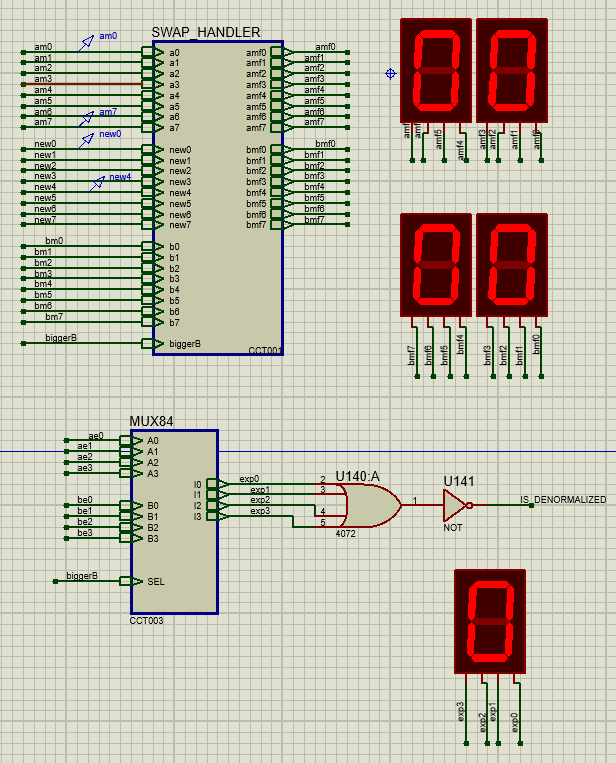
\includegraphics[scale=0.45]{swap_handler}‎
				\caption{جابه جایی ورودی ها و مشخص کردن نما و مقادیر عددی ورودی ها}
			\end{center}
		\end{figure} 
		\begin{figure}[h!]
			\begin{center}
				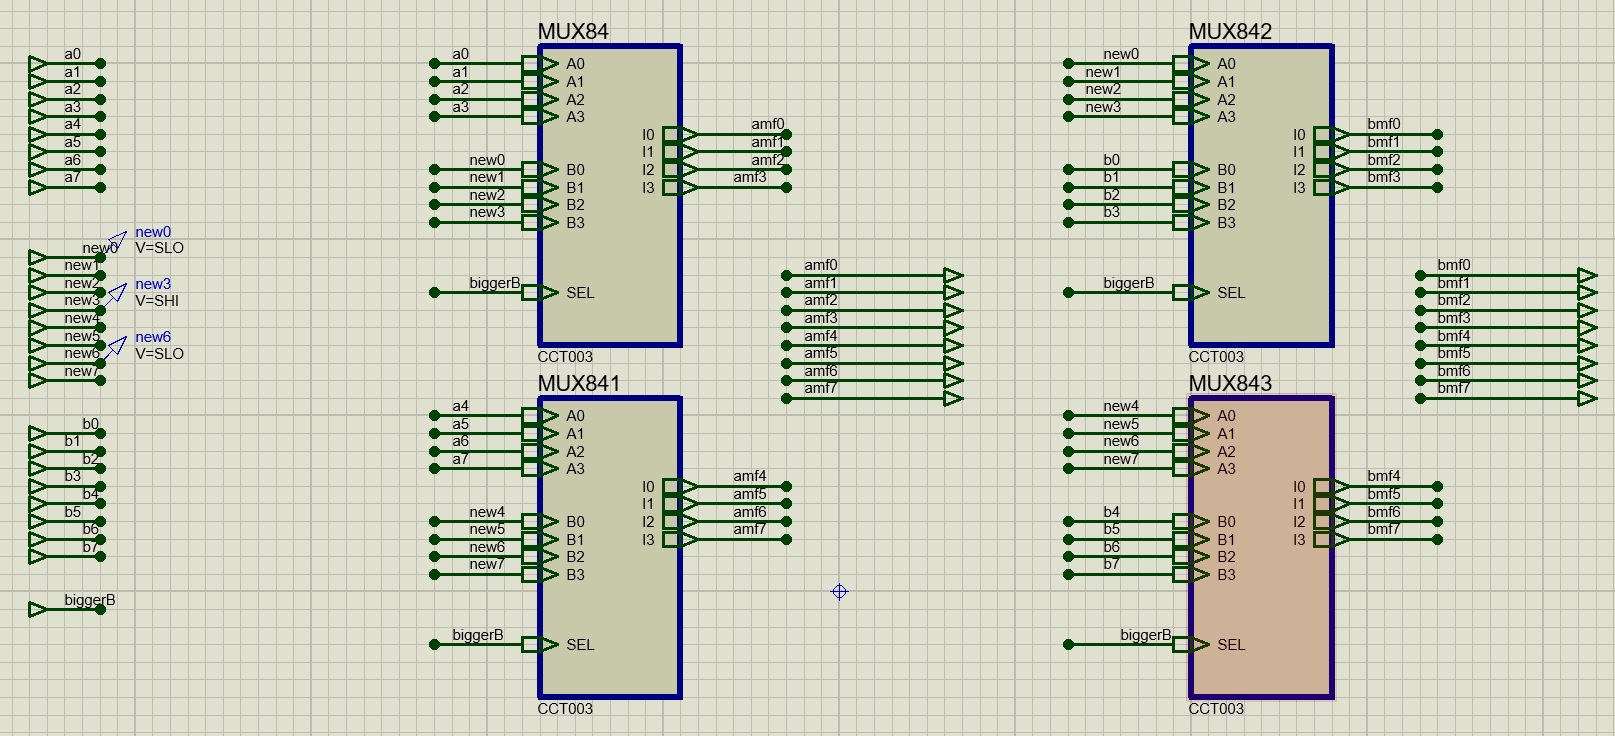
\includegraphics[scale=0.3]{swap_handler_insider}‎
				\caption{ساختار مدار جا به جا کننده}
			\end{center}
		\end{figure} 
		\item
		مقادیر align شده وارد alu میشوند تا بسته به سیگنال کنترلی add/sub محاسبه انجام شود. خروجی های alu مقدار عددی حاصل از مقایسه و علامت آن است. در صورت رخ دادن اورفلو در فرآیند جمع یا تفریق نیز سیگنال overflow فعال میشود. البته این سیگنال ارتباطی به سیگنال اورفلویی که خروجی مدار است ندارد و برای افزایش نما یه کار میرود. در مدار alu طراحی شده ابتدا در صورت منفی بودن علامت هر کدام از ورودی ها مکمل دوی آن ها محاسبه میشود و سپس وارد یک ادر 9 بیتی میشوند. در صورت رخ دادن اورفلو در جمع، سیگنال اورفلوی alu فعال میشود. خروجی 8 بیتی جمع کننده در صورتی که در جمع اورفلو رخ داده باشد، به اندازه 1 بیت به راست شیفت میخورد.
		\begin{figure}[h!]
			\begin{center}
				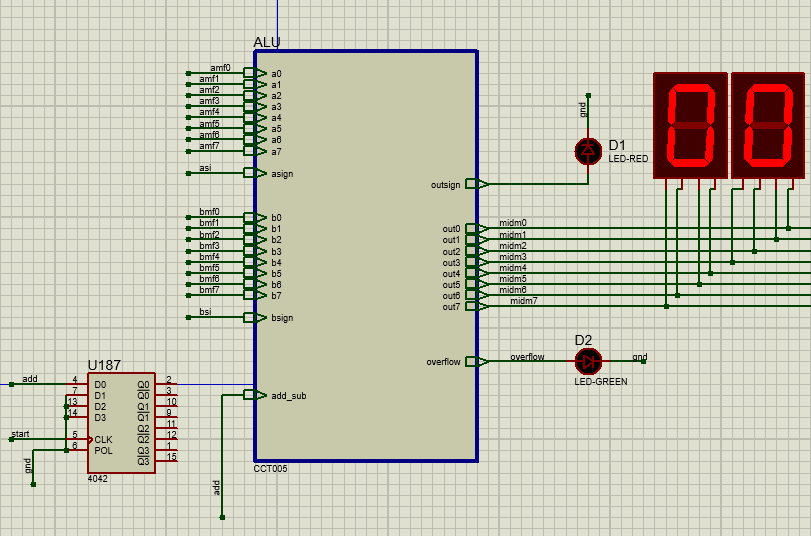
\includegraphics[scale=0.4]{alu}‎
				\caption{مدار جمع کننده/ تفریق کننده}				
			\end{center}
		\end{figure} 
		\begin{figure}[h!]
			\begin{center}
				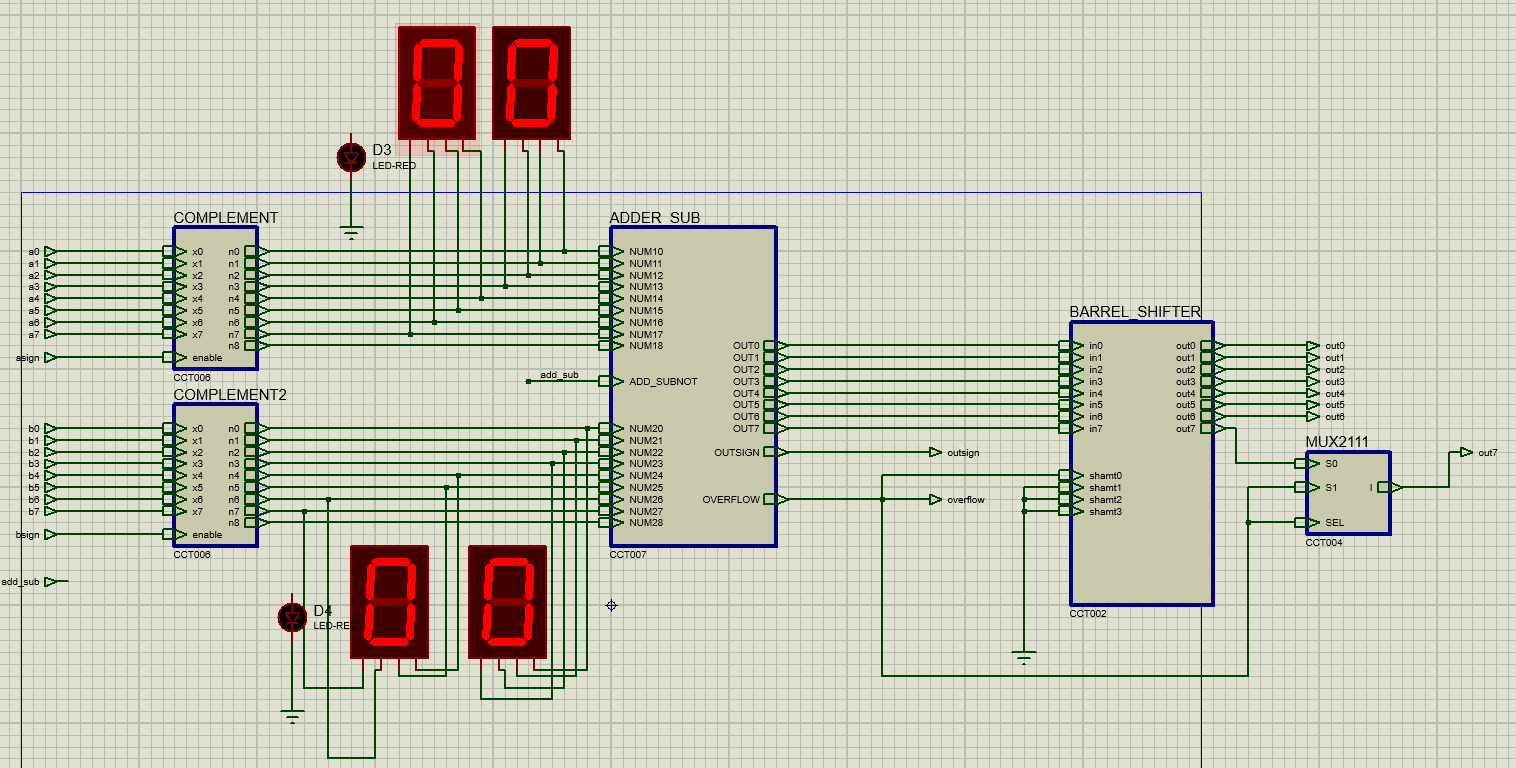
\includegraphics[scale=0.4]{alu_insider}‎
				\caption{واحد جمع کننده طراحی شده}				
			\end{center}
		\end{figure} 
		\item
		خروجی alu وارد مدار نرمالایزر میشود. و پس از نرمالایز شدن، در صورتی که خروجی نهایی نرمالایز باشد، روی خروجی های مدار قرار میگیرد.هم چنین اگر خروجی نهایی دینرمالایز باشد، خروجی نهایی از از  مدار نرمالایزر تاثیر نمی پذیرد.نمای خروجی در این قسمت تعیین میشود. در صورتی که حاصل جمع اورفلو داشته باشد، نما افزایش میابد. در صورتی که حاصل 0 باشد یا دینرمالایز باشد، نمای خروجی ازین بخش مدار 0 میشود.
		\begin{figure}[h!]
			\begin{center}
				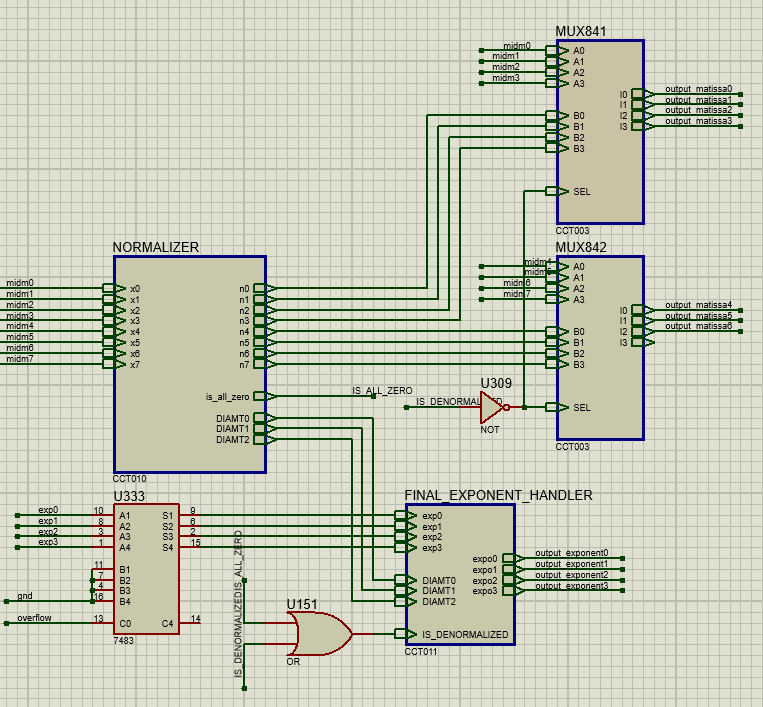
\includegraphics[scale=0.4]{normalizer}‎
				\caption{نرمالایز کردن و تعیین مانتیس و نمای خروجی مدار}
			\end{center}
		\end{figure} 
	\item
	مدار نرمالایزر طراحی شده بر پایه شمردن یک ها کار میکند. یک شمارنده LZC سریع طراحی کرده ایم که اندیس نخستین 0 عدد را خروجی میدهد و با نات کردن ورودی هایش، اندیس نخستین یک موجود در حاصل جمع یا تفریق را میابیم. در نهایت با شیفت دادن به اندازه کافی به سمت چپ، عدد را نرمالایز میکنیم به گونه ای که عدد 8 بیتی حاصل در جایگاه پرارزش خود بیت 1 داشته باشد. همچنین اگر مقدار خروجی جمع یا تفریق 0 باشد، سیگنال مربوط به 0 بودن همه بیت های مانتیس فعال میشود. این سیگنال و سیگنال تشخیص دینرمالایز همان دو سیگنالی هستند که در بخش قبلی مدار به آن ها نیاز داشتیم.
	\begin{figure}[h!]
		\begin{center}
			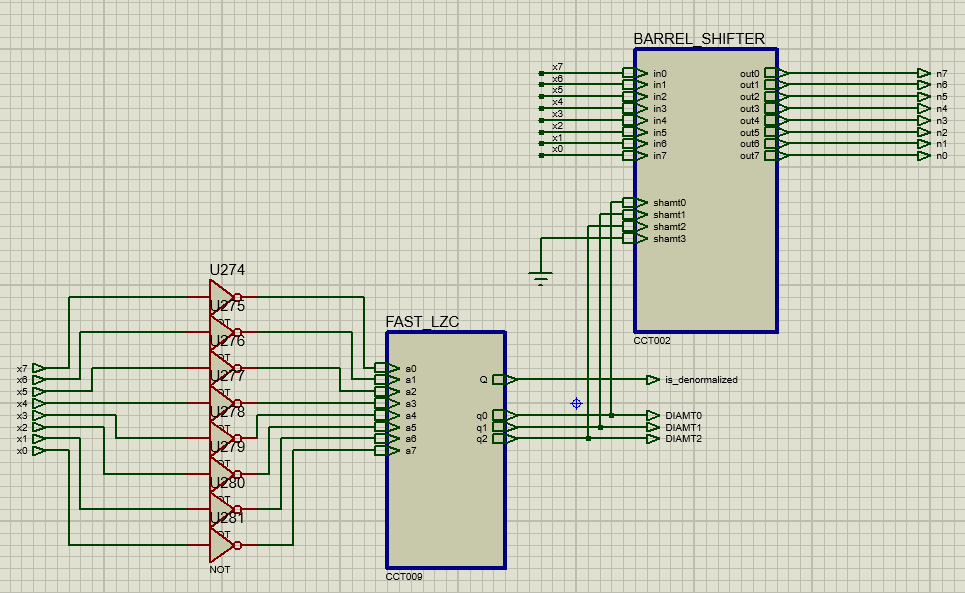
\includegraphics[scale=0.4]{normalizer_insider}‎
			\caption{مدار نرمالایزر}
		\end{center}
	\end{figure} 
	\begin{figure}[h!]
		\begin{center}
			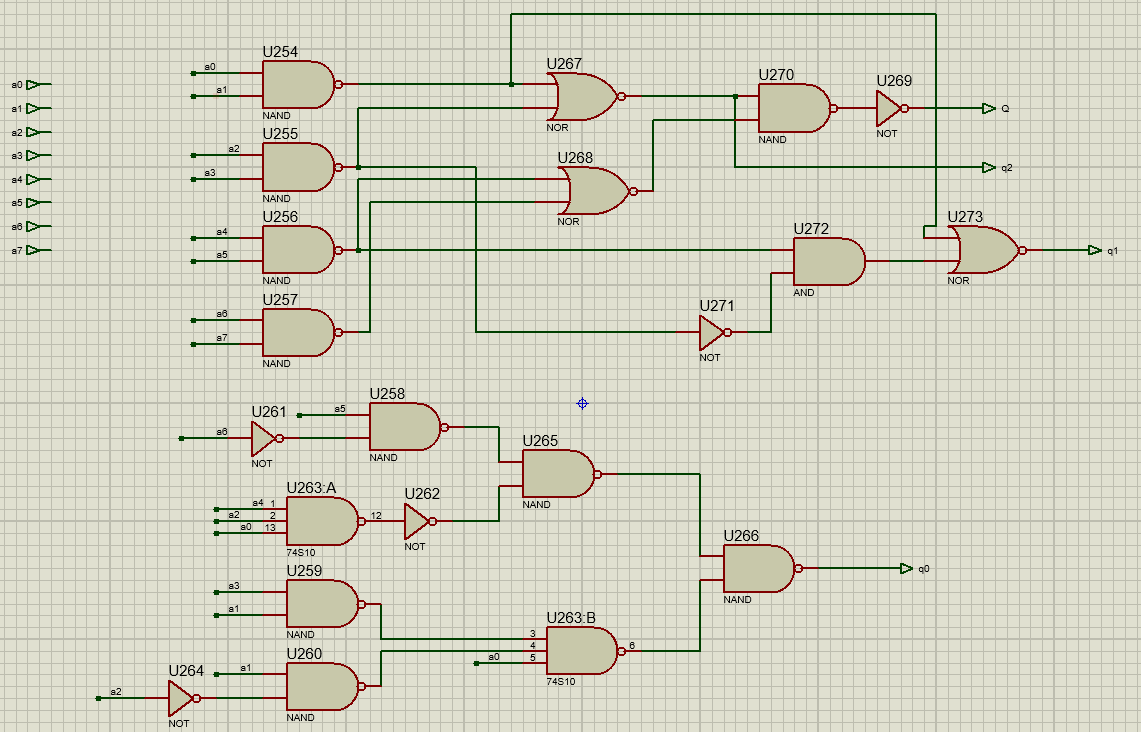
\includegraphics[scale=0.4]{lzc_insider}‎
			\caption{مدار شمارشگر صفرهای مقدم}
		\end{center}
	\end{figure} 
	
	\item
	برای ایجاد سیگنال خروجی OVERFLOW کافی است مجاز بودن نما را بررسی کنیم. در صورتی که نمای خروجی نهایی 1111 باشد اورفلو رخ داده است. همچنین برای ایجاد سیگنال خروجی END پس از گدشت دوکلاک از فعال شدن سیگنال ورودی START این سیگنال 1 میشود. با صفر شدن مجدد سیگنال START این سیگنال خروجی نیز 0 میشود.
		\begin{figure}[h!]
			\begin{center}
				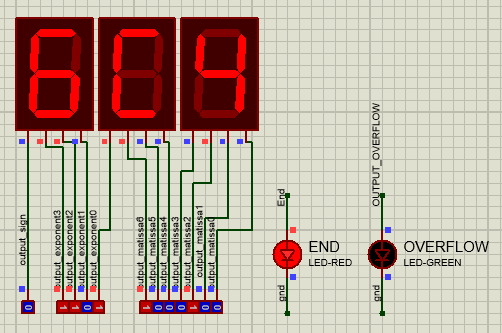
\includegraphics[scale=0.75]{outputs}‎
				\caption{خروجی های مدار}
			\end{center}
		\end{figure} 
		\newpage
	\end{itemize}

	\section*{تست و بررسی مدار برای چند ورودی متفاوت}
	\begin{itemize}
		\item
		دو ورودی A = 1AF و B = 3D7 را به مدار میدهیم و سیگنال ADD را فعال میکنیم. انتظار میرود عدد کوچکتر که همان A است به اندازه 4 واحد به راست شیفت بخورد تا مقادیر align شوند. در نهایت حاصل جمع برابر با مقدار عددی E1 و نمای 7 خواهد شد. نمایش ممیز شناور این عدد به صورت 3E1 خواهد بود.
		\begin{figure}[h!]
			\begin{center}
				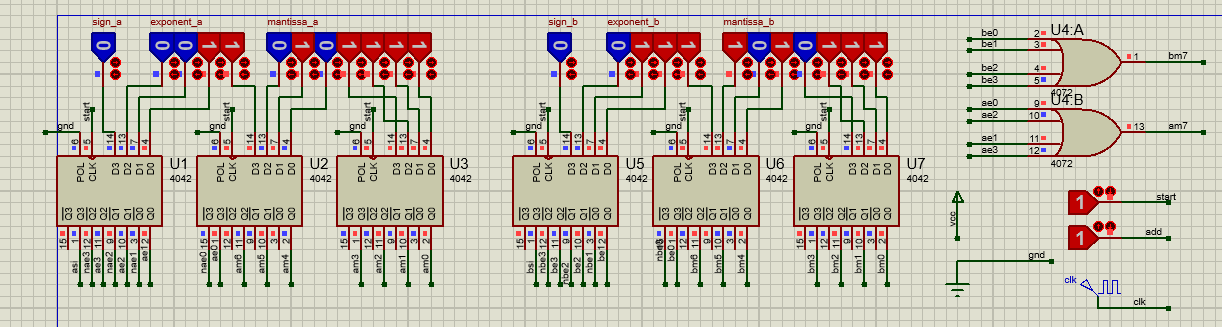
\includegraphics[scale=0.5]{test1_inputs}‎
				\caption{ورودی های تست اول}
			\end{center}
		\end{figure} 
	\begin{figure}[h!]
		\begin{center}
			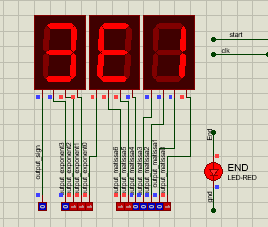
\includegraphics[scale=0.8]{test1_outputs}‎
			\caption{خروجی های های تست اول}
		\end{center}
	\end{figure} 
		\item
				دو ورودی A = 28F و B = 2F0 را به مدار میدهیم و سیگنال ADD را غیرفعال میکنیم. نمای هر دو عدد برابر است پس align تغییر خاصی در ورودی ها نمیدهد. انتظار میرود حاصل تفریق منفی مقدار عددی 61 باشد و خروجی ممیز شناور حاصل A42 باشد.
			\begin{figure}[h!]
				\begin{center}
					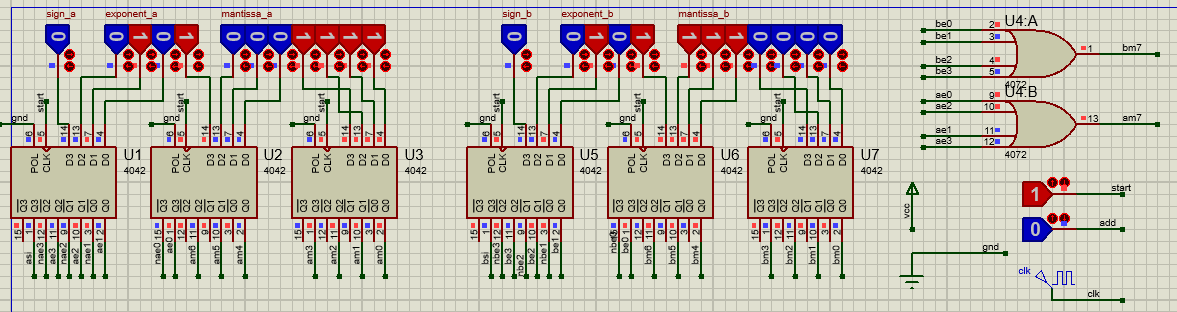
\includegraphics[scale=0.5]{test2_inputs}‎
					\caption{ورودی های تست دوم}
				\end{center}
			\end{figure} 
			\begin{figure}[h!]
				\begin{center}
					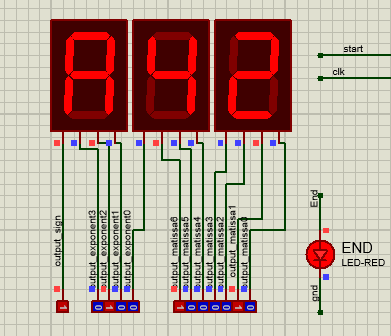
\includegraphics[scale=0.8]{test2_outputs}‎
					\caption{خروجی های های تست دوم}
				\end{center}
			\end{figure} 
	\end{itemize}
	
	\newpage
	\section*{لیست قطعات و تراشه های استفاده شده برای طراحی مدار}
	\begin{figure}[h!]
		\begin{center}
			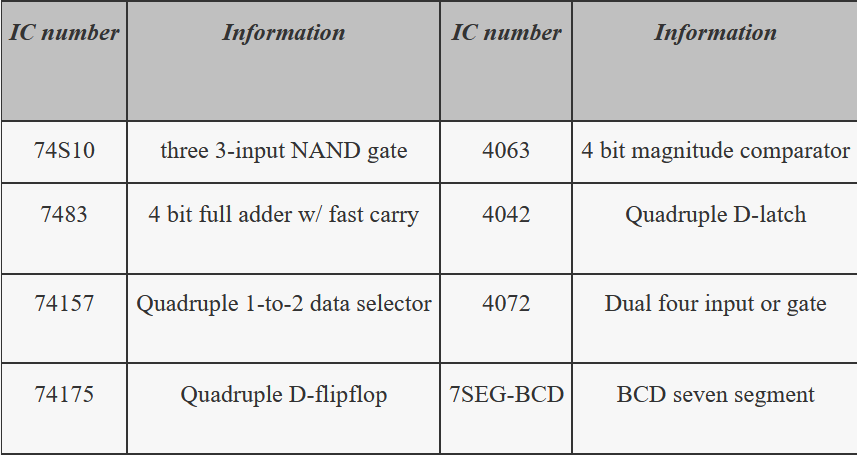
\includegraphics[scale=0.43]{ics}‎
			\caption{تراشه های به کار رفته در مدار}
		\end{center}
	\end{figure} 
	
\end{document}









